\documentclass[11pt]{article}

% ---------- Packages ----------
\usepackage[margin=1in]{geometry}
\usepackage{amsmath, amssymb}
\usepackage{graphicx}
\usepackage{fancyhdr}
\usepackage{float}
\usepackage{listings}

% ---------- MATLAB Code Listing Style ----------
\lstdefinestyle{matlab}{
    language=Matlab,
    basicstyle=\ttfamily\footnotesize,
    breaklines=true,
    breakatwhitespace=false,
    postbreak=\mbox{$\hookrightarrow$\space},
    columns=fullflexible,
    keepspaces=true,
    frame=none,
    numbers=left,
    numberstyle=\tiny,
    showstringspaces=false
}
\lstset{style=matlab}

% ---------- Paragraph Formatting ----------
\setlength{\parindent}{0pt}
\setlength{\parskip}{0.5em}

% ---------- Header ----------
\pagestyle{fancy}
\fancyhf{}
\lhead{ASEN 5335 Aerospace Environment}
\rhead{Justin Le}
\cfoot{\thepage}

% ---------- Document ----------
\begin{document}

% ---------- Title ----------
\begin{center}
    {\Large \textbf{Homework 2}}\\[0.5em]
    {\large ASEN 5335 Aerospace Environment}\\[0.5em]
    Justin Le\\ 
    \today
    \\[0.5em]
\end{center}

\vspace{1em}
\section*{Problem 1: Plotting the Ionosphere}
\subsection*{(i.)}

\begin{figure}[H]
    \centering
    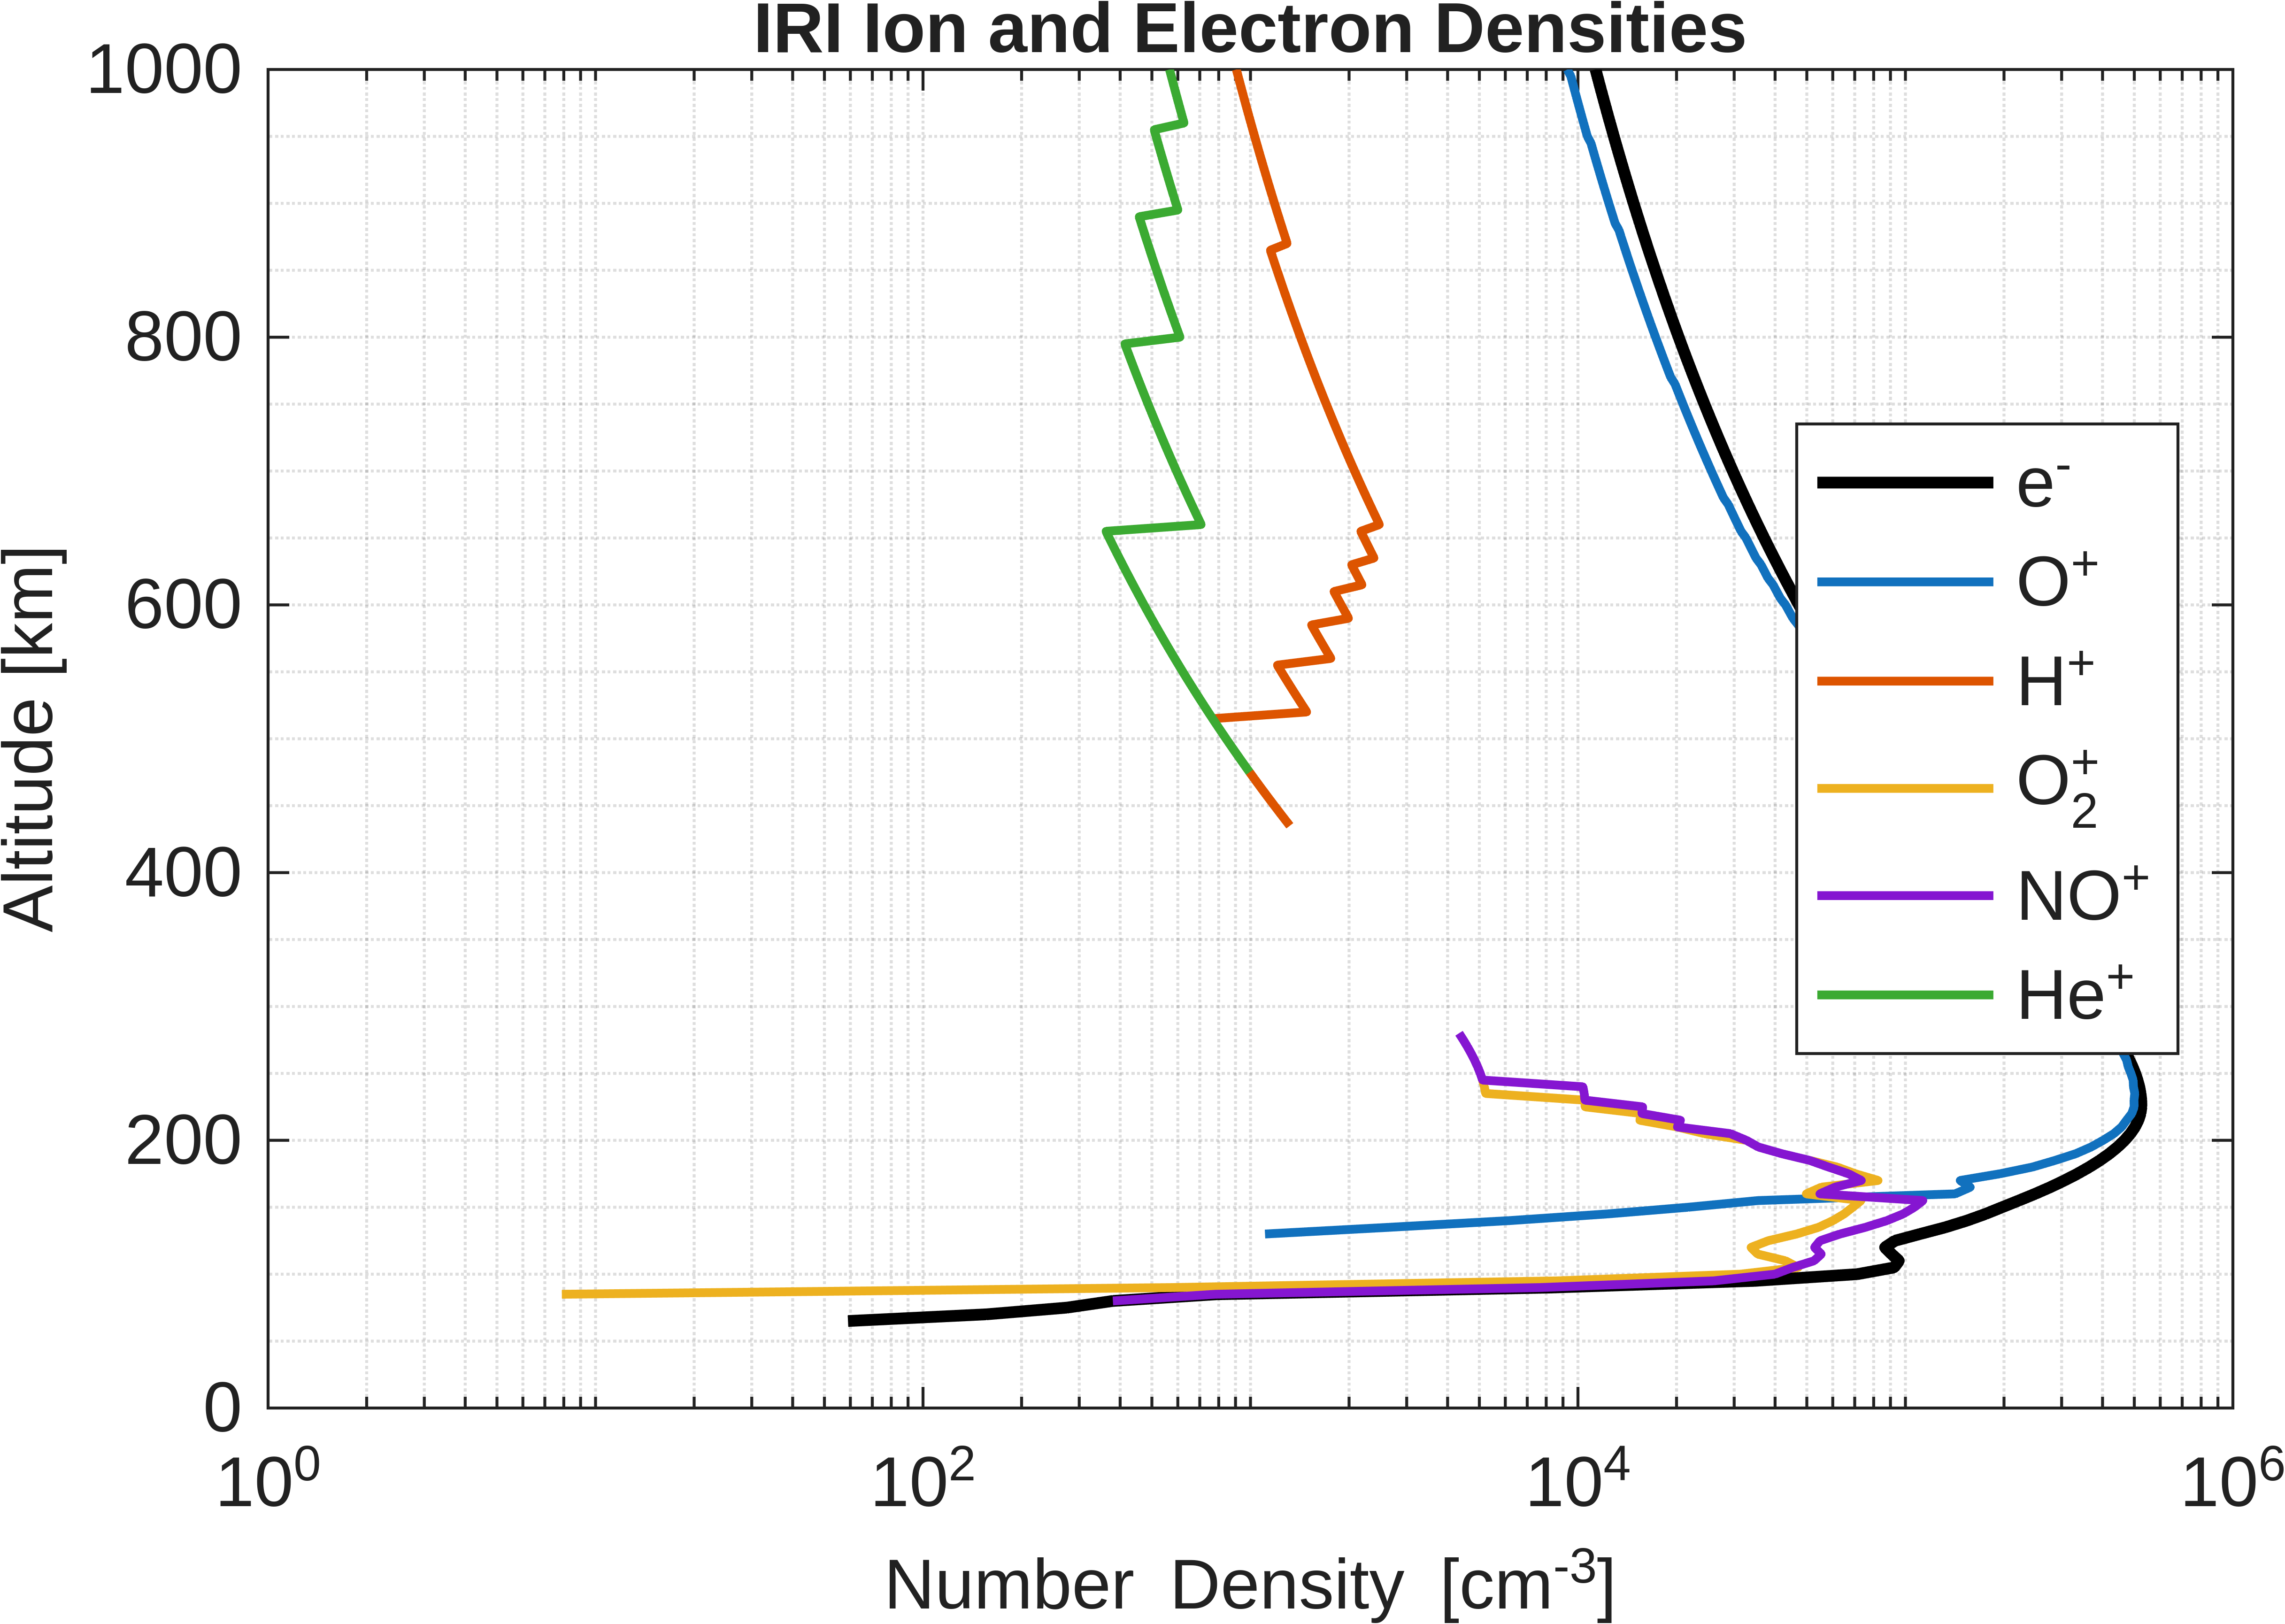
\includegraphics[width=0.6\textwidth]{figures/HW3_P1_iri_output.png}
    \caption{IRI Output}
    \label{fig:iri_output}
\end{figure}

\begin{figure}[H]
    \centering
    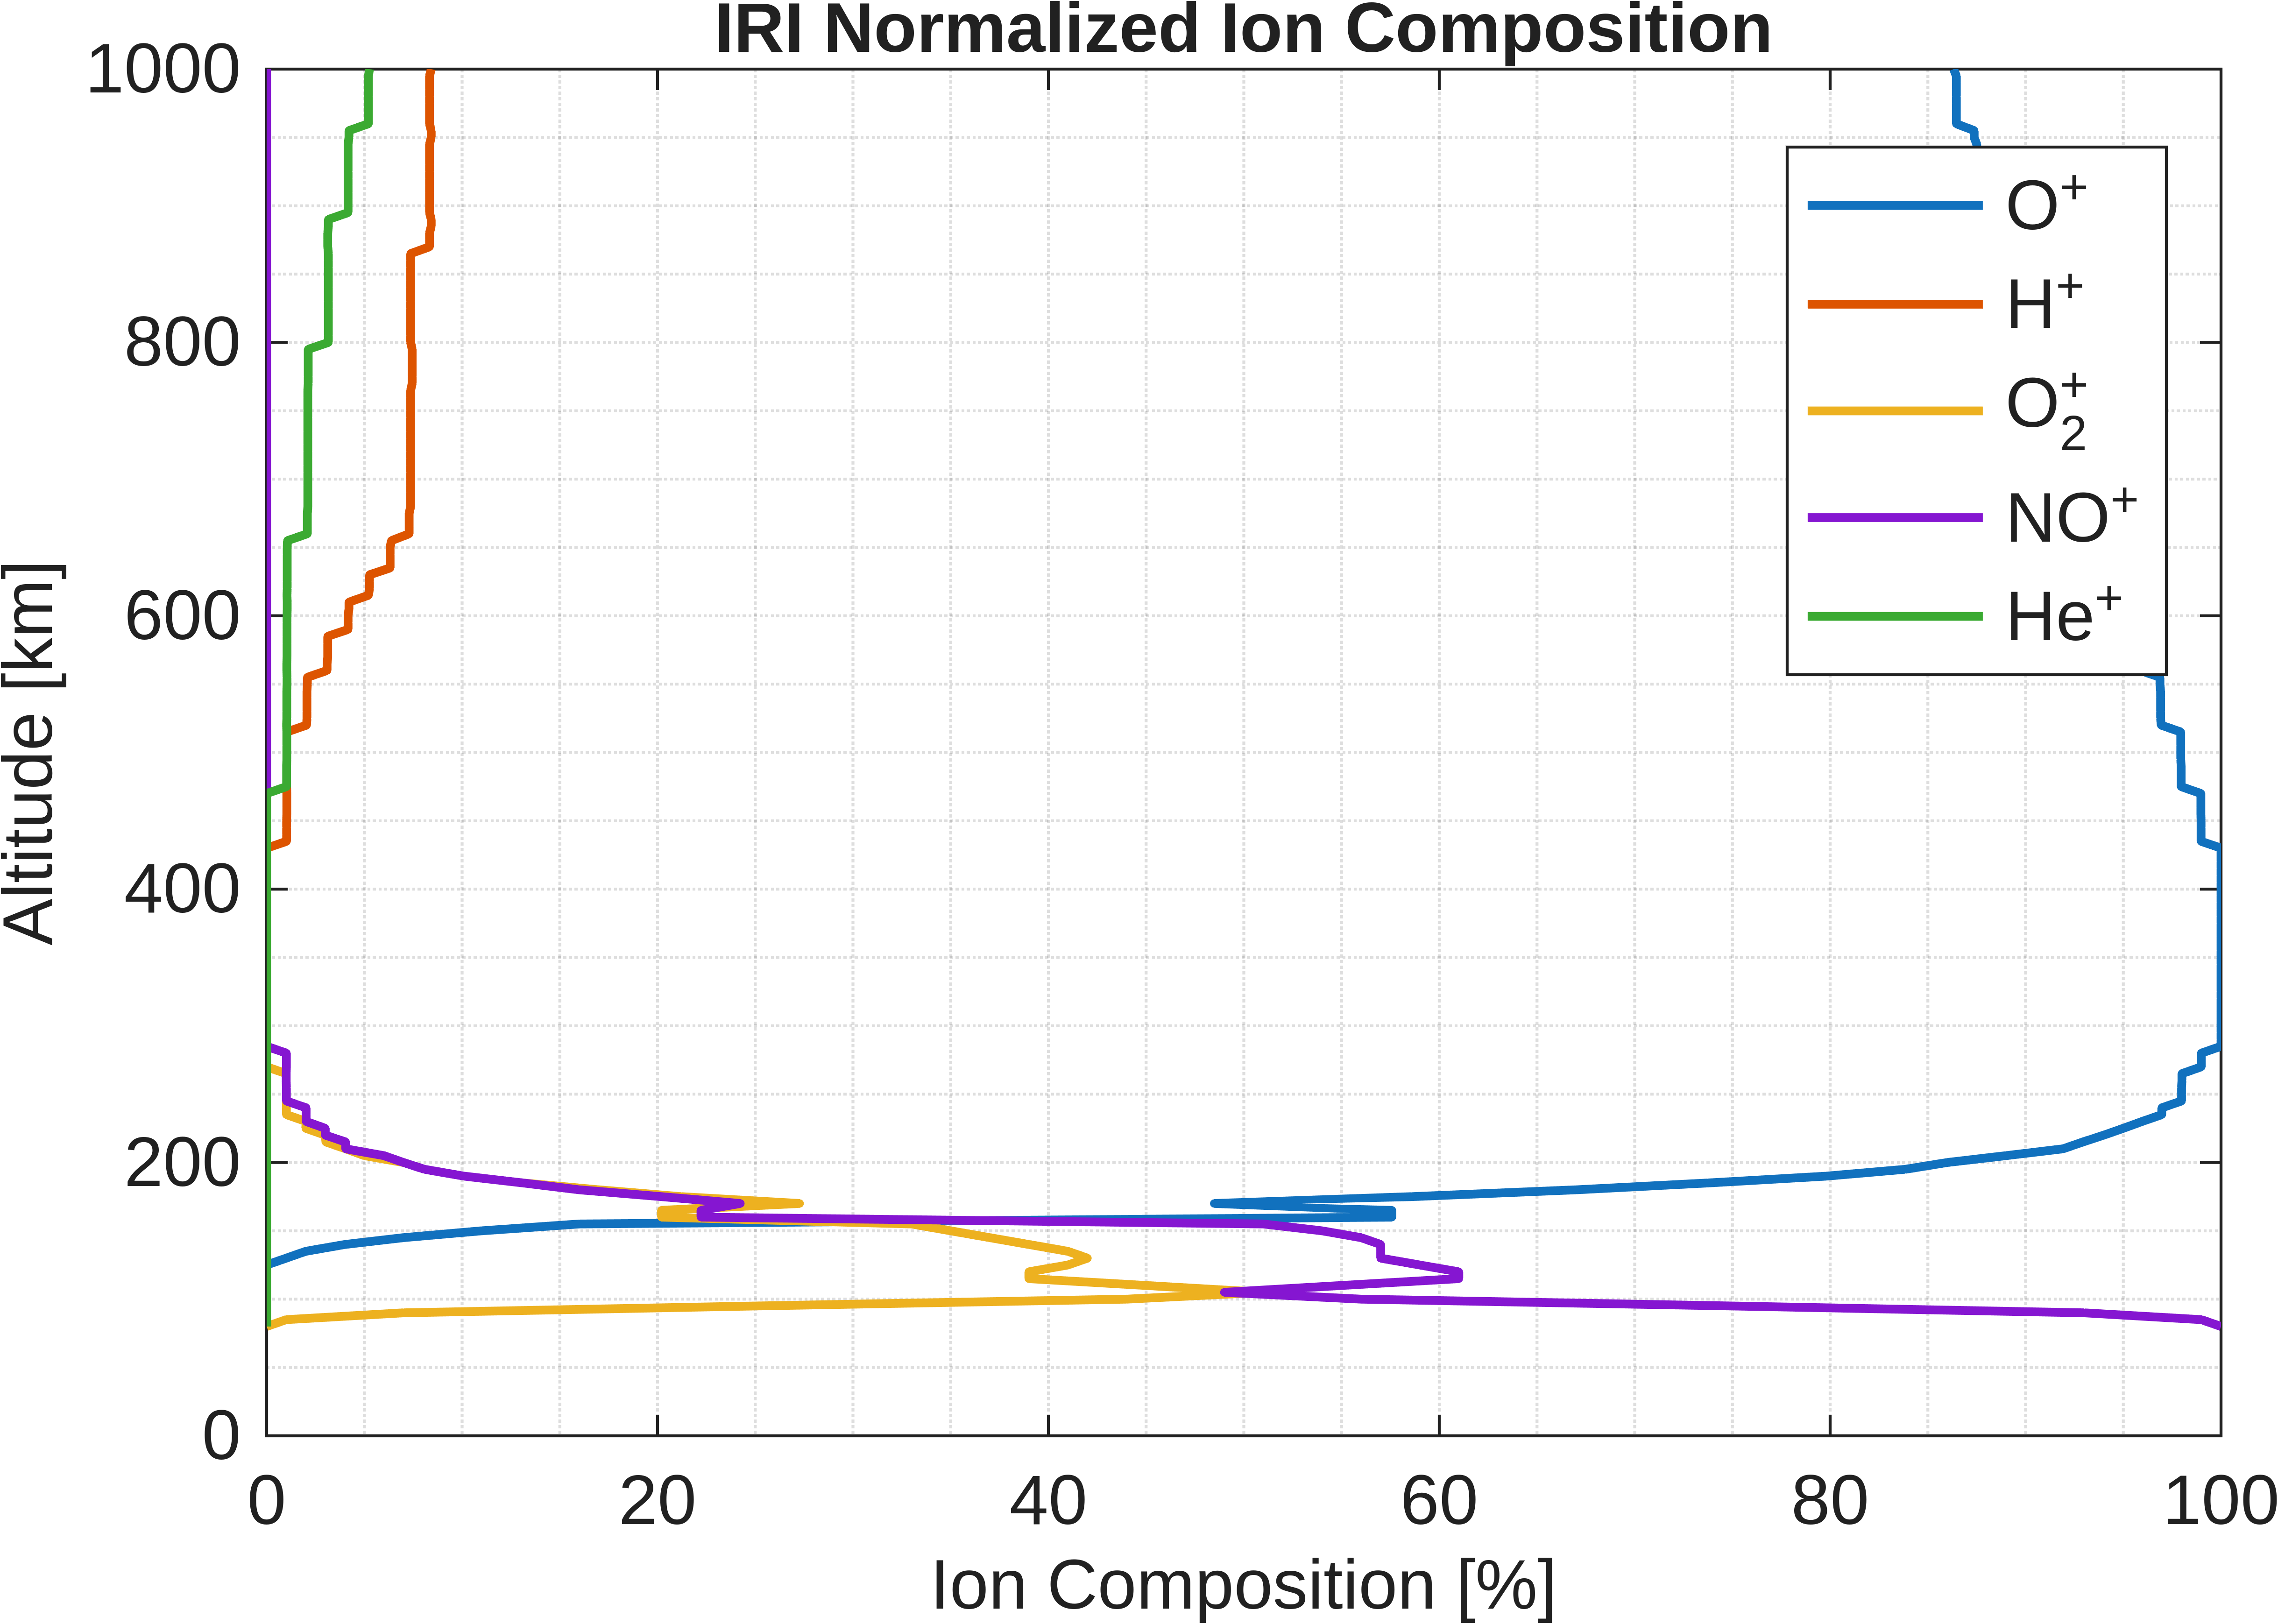
\includegraphics[width=0.6\textwidth]{figures/HW3_P1_ion_composition.png}
    \caption{IRI Output Normalized}
    \label{fig:iri_output_normalized}
\end{figure}

\subsection*{(ii.)}
\hspace*{2em}Below 500 km, we can observe that $NO^+$ dominates between 0-160 km. $O_2^+$ contributes more than 20\% at
between 90 and 175 km. 

\subsection*{(iii.)}
\hspace*{2em}By convention 1 TECU is $10^{16}\,\mathrm{el/m^2}$. Integrating the total electrons from the IRI
output, we find the TEC of the entire IRI output to be 12.47 TECU. When the peak electron density is $525696\,\mathrm{m^{-3}}$, we can integrate
the topside and bottomside seperately to find they are 3.55 TECU and 8.92 TECU respectively. Normalizing against the total TEC found, we find they are
28.49\% and 71.51\% respectively. 

\newpage
\section*{Problem 2: Peak Ionization}

\newpage
\section*{Problem 3: Spacecraft Charging in LEO}

\newpage
\section*{Problem 4: Spacecraft Charging in GEO}

\newpage
\section*{Problem 5: Radio Wave Propagation}

\newpage
\section*{Problem 6: Radio Blackout}

\newpage
\section*{Problem 7: GPS Delays}

\newpage
\section*{Problem 8: D Region Signal Attenuation}

\newpage
\section*{Problem 9: ICON Mission}

\end{document}
